\chapter{Training e Test del BDT}



\section{Training}

In questa sezione verr\`a descritta la fase di training del metodo di analisi multivariata del Boosted Decisione Tree (BDT), in particolare: il campione di dati che \`e stato utilizzato per il training, le variabili discriminatorie utilizzate come input per il BDT per separare il segnale dal fondo e la scelta dei parametri di configurazione del BDT. 

\subsection{Campione di dati per il training}
Come detto nel capitolo precedente per la fase di training del BDT è necessario un insieme di dati di cui sia nota la distinzione tra segnale e fondo. 

Per il segnale è stato utilizzato un campione di dati ottenuto da una simulazione Monte Carlo,  in cui vengono generate collisioni protone-protone all'energia del centro di massa di 5~TeV e i mesoni D*+ prodotti vengono forzati a decadere nel canale di decadimento di interesse. In questo modo \`e certa l'identi\`a della candidata $D^{*+}$.
\\Al contrario, il campione di candidate per il fondo combinatoriale \`e stato selezionato dai dati raccolti da Alice\cite{dati_ALICE} (collisioni protone-protone a 5~TeV nel centro di massa) considerando candidate con valori della differenza tra la massa invariante della $D^{*+}$ e della $D^0$: $\Delta M > 147.8$ MeV/$c^2$  e $\Delta M < 143.0$ MeV/$c^2$, cio\`e candidate a destra e a sinistra del picco a 145 MeV/$c^2$ nella distribuzione di $\Delta M$ mostrata in figura \ref{fig:grafmassDstar2}. In questo modo si considerano i dati a circa $4 \sigma$ della Gaussiana che descrive il picco del segnale e si pu\`o essere sicuri di non includere anche parte del segnale.
\\Si \`e scelto di utilizzare i dati stessi invece che una simulazione Monte Carlo in quanto \`e importante che il campione per il training sia il pi\`u possibile simile al campione da utilizzare. Il fondo preso dal Monte Carlo presenta delle differenze nella distribuzione delle variabili discriminatorie tali da non permettere una buona separazione tra segnale e fondo.

L'analisi \`e stata svolta in diversi intervalli di impulso trasverso ($p_T$) delle candidate $D^{*+}$. L'impulso trasverso \`e l'impulso nella direzione perpendicolare ai fasci di protoni incidenti. Gli intervalli considerati sono [0,1], [1,2], [2,3], [3,4], [4,5], [5,6], [6,8], [8,12], [12,16], [16,24] misurati in GeV/c. 
\\In figura \ref{fig:dati_training} è riportata la distribuzione di massa invariante $\Delta M = M(K,\pi,\pi)-M(K,\pi))$ dei campioni di segnale e fondo utilizzati per il training del BDT. 

    \begin{figure}[htbp] 
        \centering
        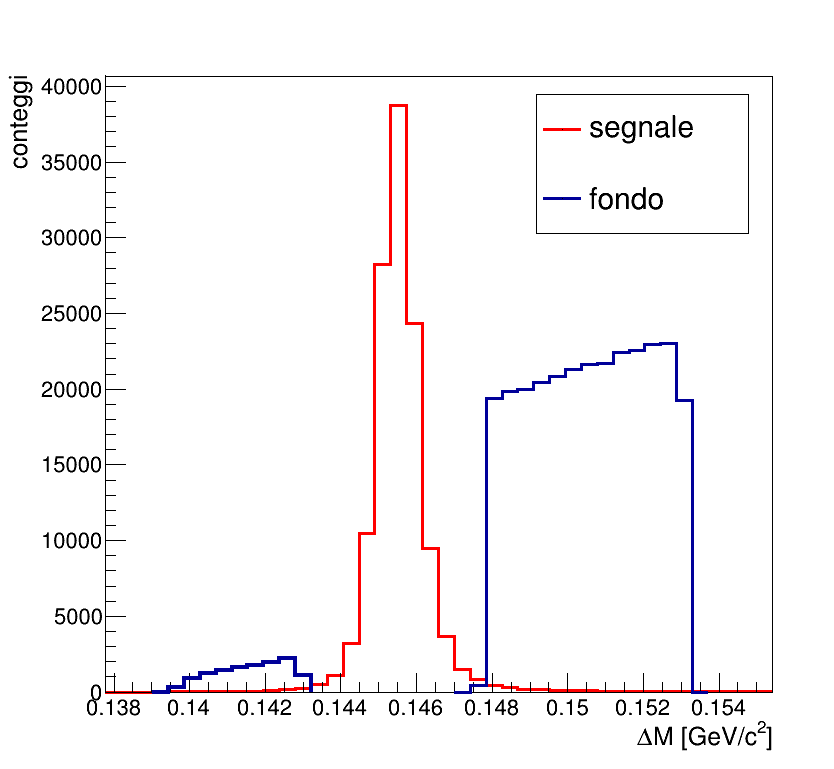
\includegraphics[width=0.7\linewidth]{training&testing/dati_training.png}
        \caption{Distribuzione di massa invariante $\Delta M = M(K,\pi,\pi)-M(K,\pi)$ dei campioni di dati utilizzati per il training per l'intervallo di $p_T$ [3-4] GeV/c. In rosso \`e mostrato il campione di segnale ottenuto dalla simulazione Monte Carlo, in blu il fondo combiantoriale selezionato dai dati di ALICE.}
        \label{fig:dati_training}
    \end{figure}
    
La tabella \ref{Tab:dati_training} riporta la quantità di dati per il segnale e per il fondo utilizzati per il training in ogni intervallo di $p_T$. 
 
      \begin{table}[H]
		\centering
		\captionof{table}{Dati utilizzati per il training.\label{Tab:dati_training}}
		\begin{tabular}{c|c|c}
		    \toprule
		    $D^{*+}$ $p_T$ [GeV/c]  &  numero candidate $D^{*+} $ & numero combinazioni non \\& per il segnale &relative alla $D^{*+}$ per il fondo \\
            \midrule
            1 - 2  	&  10000   &  100000  \\ 
            2 - 3 	&  30000   &  90000  \\
            3 - 4  	&  30000   &  30000  \\ 
            4 - 5  	&  20000   &  10000 \\ 
            5 - 6  	&  17000   &  4000  \\ 
            6 - 8  	&  20000   &  2800  \\ 
            8 - 12  &  12000   &   900 \\   
			\bottomrule
		\end{tabular}
	\end{table}
	
Come \`e possibile vedere dalla tabella, il numero di eventi di fondo selezionati diminuisce al crescere del $p_T$. Questo e' dovuto ad una naturale diminuzione del fondo combinatoriale al crescere del $p_T$ della candidata $D^{*+}$. A causa del numero limitato di eventi di fondo disponibili per il training del modello, non e' stato possibile estendere l'analisi ad intervalli di impulso pi\`u alto. Infatti, come si vede dalla tabella, gi\`a nell'intervallo di $p_T&$ 8-12 GeV/c sono disponibili solo 900 eventi di fondo e solo 500 eventi di fondo erano disponibili per $p_T$ > 12 GeV/c. Infine, non e' stato possibile estendere l'analisi a $p_T < 1$ GeV/c perch\`e le D*+ con impulso $p_T < 1$ GeV/c erano state rigettate nel Monte Carlo considerato.

\subsection{Variabili discriminatorie per il training}
L'analisi svolta in questa tesi \`e basata sullo studio del decadimento $D^{*+} \rightarrow D^0( \rightarrow K^- \pi^+)  \pi^+ $ attraverso l'utilizzo di metodi di analisi multivariati, basati sull'analisi combinata di pi\`u variabili, definite variabili discriminatorie. %In particolare si \`e usato il metodo del Boosting Decision Tree implementato nel TMVA di Root. 
\\Le variabili discriminatorie che sono state considerate sono quelle che vengono generalmente utilizzate nell'analisi standard\cite{dati_ALICE} e includono le variabili gi\`a mostrate nel paragrafo \ref{mesoneD} e nella figura \ref{fig:decadimentoD}:       \begin{enumerate}
 \item la distanza minima tra la traiettoria del Kaone $K^-$  e il vertice primario (PV) (\textbf{d0K});
                \item la distanza minima tra la traiettoria del $\pi^+$ (prodotto dal decadimento della $D^0$) e il PV (\textbf{d0Pi});
            \item la distanza minima tra le traiettorie del $K^-$ e del $\pi^+$ (\textbf{DCA});
            \item il coseno dell'angolo di puntamento, ovvero l'angolo tra la retta congiungente il PV e il vertice secondario (SV) e la direzione del $p_T$ della $D^{*+}$ (\textbf{cosThetaPoint});
            e la sua proiezione sul piano perpendicolare alla direzione dei fasci di protoni (\textbf{cosThetaPointXY});
            \item la lunghezza di decadimento delle candidate $D^0$, ovvero la distanza di volo della $D^0$, normalizzata per il suo errore (\textbf{NormDecayLenght}) e la  proiezione sul piano perpendicolare alla direzione del fascio (\textbf{NormDecayLenghtXY});
            \item il prodotto delle distanze minime tra le traiettorie del  $K^-$ e del $\pi^+$ dal PV (\textbf{d0d0});
            \item l'impulso del $\pi^+_{soft}$ (prodotto dal decadimento della $D^{*+}$) nella direzione perpendicolare a quella del fascio (\textbf{softPiPt})
            \item l'impulso del $\pi^+$ (prodotto dal decadimento della $D^0$) nella direzione perpendicolare a quella del fascio (\textbf{pTpi});
            \item l'impulso del $K^-$ nella direzione  perpendicolare a quella del fascio (\textbf{pTK});
            \item la pseudorapidit\`a del $\pi_{soft}$ (\textbf{Pieta});
            \item l'angolo tra il vettore impulso delle candidate $D^0$ e il vettore impulso del $\pi^+$ nel sistema di riferimento della $D^0$ (\textbf{cosThetaStar}) e \textbf{cosThetaStarBar} che \`e lo stesso angolo considerando le rispettive antiparticelle;
            \item l'angolo tra la direzione dell'impulso del $\pi_{soft}$ e il piano individuato dagli impulsi del $K^-$ e del $\pi^+$ (\textbf{theta}).
            
        \end{enumerate}
       

I grafici in figura \ref{fig:variabili_discr} riportano le distribuzioni di quattro delle variabili discriminatorie sopra riportate, scelte a titolo esemplificativo, per il campione di dati ottenuto da simulazione Monte Carlo utilizzato per il training del segnale, per il campione di dati di ALICE negli intervalli di massa invariante $\Delta M > 147.8$ MeV/$c^2$  e $\Delta M < 143.0$ MeV/$c^2$ utilizzato per il training del fondo e per i dati di ALICE che verranno analizzati. Da questi grafici si può vedere che le variabili discriminatorie hanno una distribuzione diversa nel caso si consideri il segnale o il fondo e sfruttando queste differenze il BDT combina le variabili discriminatorie assieme fornendo la variabile di output che permetterà poi di separare il segnale dal fondo. 
   
   \begin{figure}
       \centering
       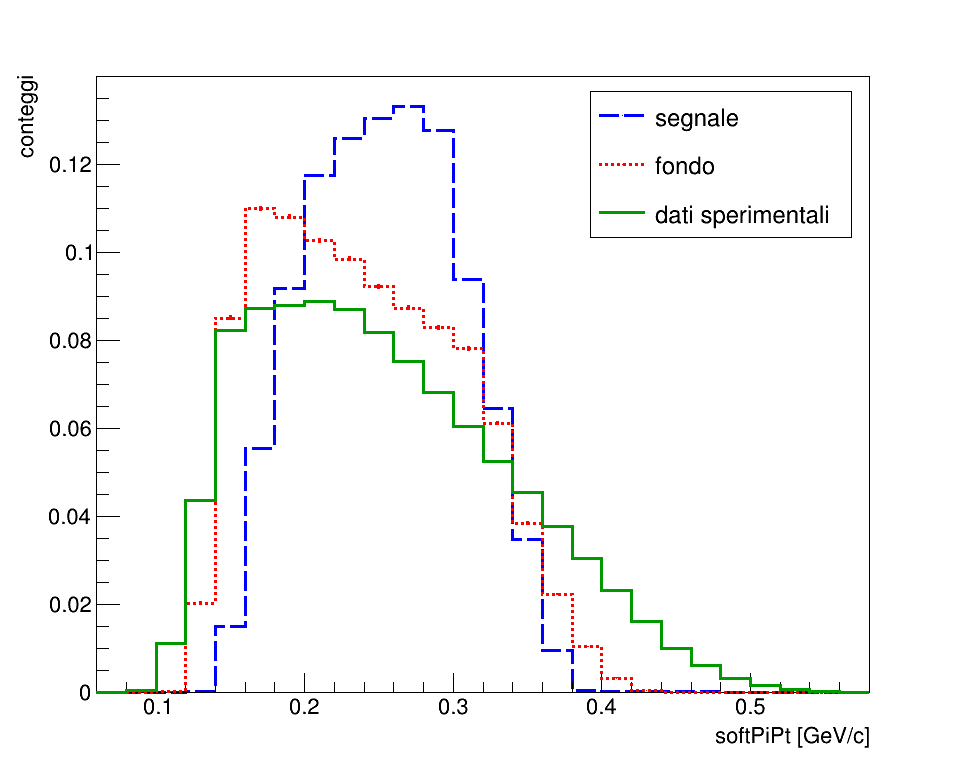
\includegraphics[width=0.48\textwidth]{training&testing/softPiPt_DBS.png}
        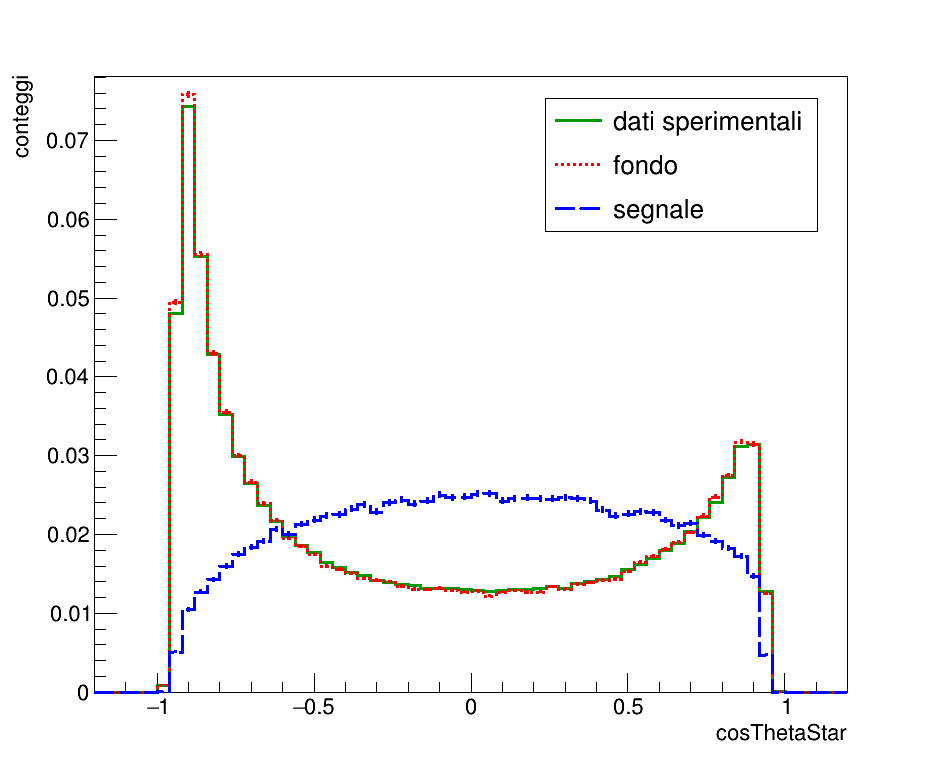
\includegraphics[width=0.48\textwidth]{AnalisiDati/cosTehtaStar_DBS.png}\\
        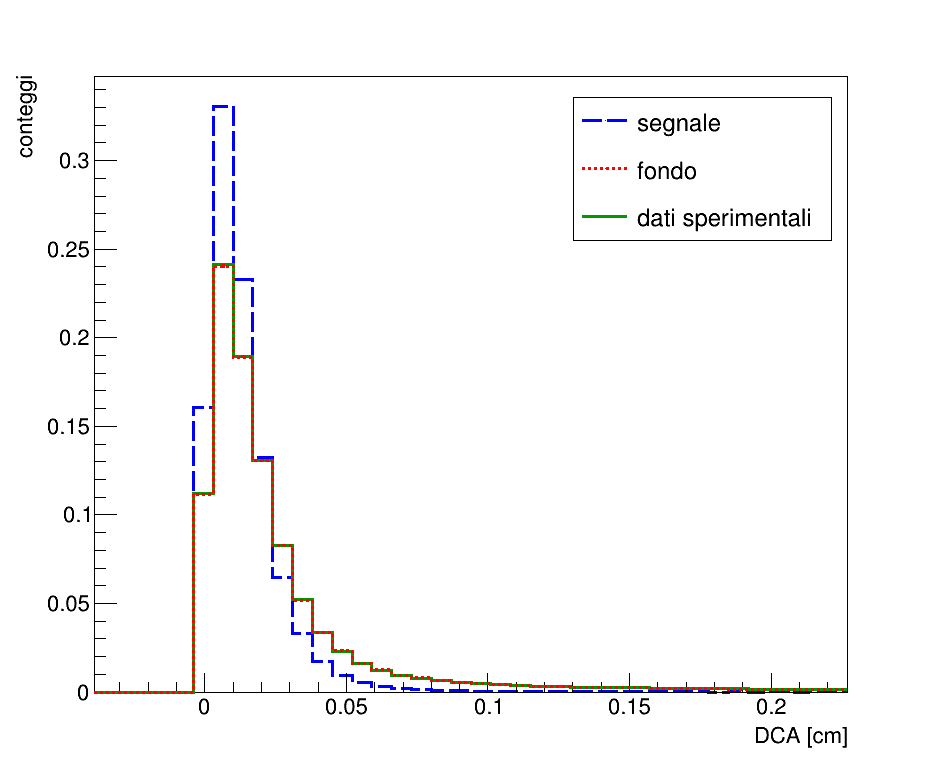
\includegraphics[width=0.48\textwidth]{training&testing/DCA_DBS.png}
        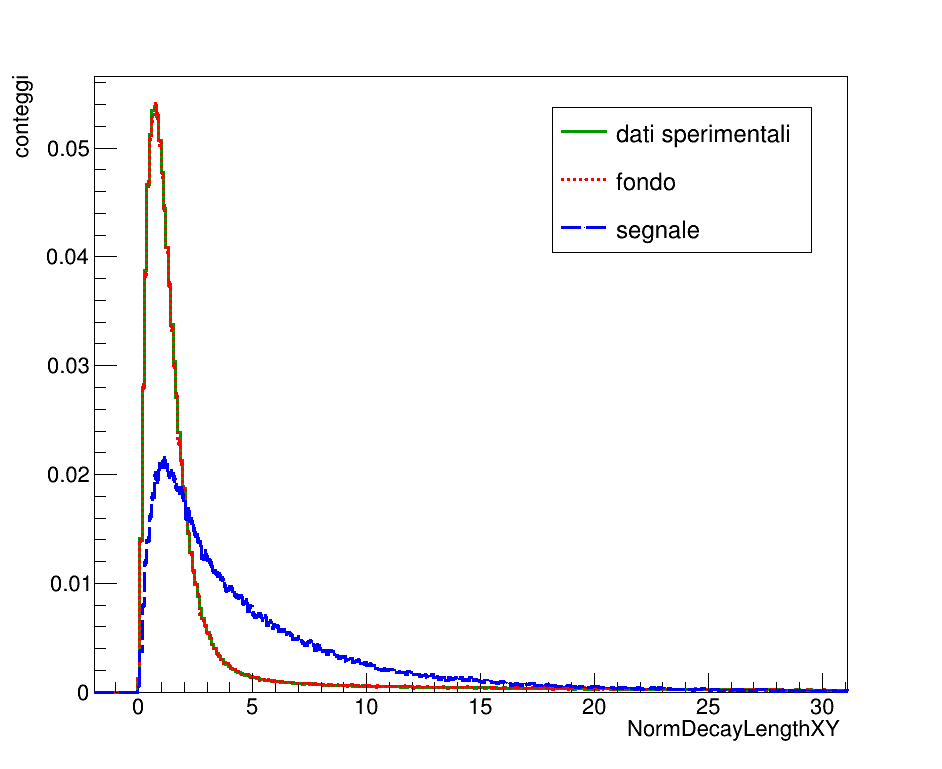
\includegraphics[width=0.48\textwidth]{training&testing/NormDecayLengthXY.png}
       \caption{Distribuzione di alcune variabili discriminatorie usate come input per il BDT,  in rosso per il campione di dati utilizzato per il training del fondo, in blu per il campione di dati utilizzato per il training del segnale e in verde per i dati di ALICE.}
       \label{fig:variabili_discr}
   \end{figure}
   
 
 
% \iffalse
%    \fi 
    
    Tra le variabili discriminatorie sono state introdotte le variabili legate all'identificazione delle particelle (PID) tramite la perdita di energia per ionizzazione $\frac{dE}{dx}$ nella TPC e tramite la misura del tempo di volo dal punto in cui si è formata la particella al rivelatore Time-Of-Flight (TOF).
    \\In figura \ref{fig:BBnellaTPC} è riportata la distribuzione della perdita di energia per ionizzazione misurata dal rivelatore TPC per le particelle cariche prodotte in collisioni protone-protone con energia nel centro di massa $\sqrt{s} = 7 $ TeV, che è confrontata con l'andamento teorico determinato dalla curva di Bethe-Bloch per le diverse particelle.
    \\ Le variabili discriminatorie relative alla PID utilizzate sono:
        \begin{enumerate}[resume]
            \item la differenza tra la perdita di energia per ionizzazione misurata dalla TPC e la perdita di energia teorica determinata con la Bethe-Bloch per il $\pi^+$ prodotto dal decadimento della $D^0$: $n\sigma_{(\pi^+,TPC)}/\sigma_{TPC} = (\frac{dE}{dx}\mid_{m, \pi} \ - \ \frac{dE}{dx}\mid_{th, \pi} ) / \sigma_{TPC} \ $ dove $ \ \sigma_{TPC}$ è la risoluzione della Time-Projection-Chamber (\textbf{nSigmaTPCpi})
            \item la differenza tra la perdita di energia per ionizzazione misurata dalla TPC e la perdita di energia teorica data dalla Bethe-Bloch per il $K^-$: $n\sigma_{(K^-,TPC)}/\sigma_{TPC} = (\frac{dE}{dx}\mid_{m,K} \ - \ \frac{dE}{dx}\mid_{th,K} ) / \sigma_{TPC} \ $ (\textbf{nSigmaTPCK})
            \item la differenza tra il tempo di volo misurato dal rivelatore Time-Of-Flight e il tempo di volo teorico per il  $\pi^+$ prodotto dal decadimento della $D^0$: $ n\sigma_{(\pi^+,TOF)}/\sigma_{TOF} = (t_{TOF}\mid_{m,\pi} \ - \ t_{TOF}\mid_{th,\pi}) / \sigma_{TOF} \ $ dove $\sigma_{TOF}$ è la risoluzione del rivelatore Time-Of-Flight (\textbf{nSigmaTOFpi})
            \item la differenza tra il tempo di volo misurato dal rivelatore Time-Of-Flight e il tempo di volo teorico per il  $K^-$: $n\sigma_{(K^-,TOF)}/\sigma_{TOF} = (t_{TOF}\mid_{m,K} \ - \ t_{TOF}\mid_{th,K})\sigma_{TOF} \ $ (\textbf{nSigmaTOFK})
        \end{enumerate}
    
        
   
   \begin{figure}[htbp]
        \centering
        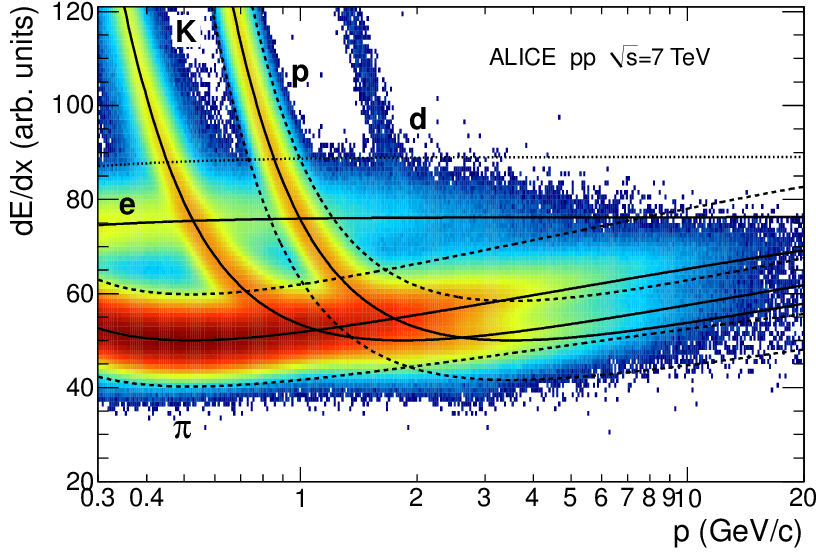
\includegraphics[width=0.7\linewidth]{training&testing/Specific-energy-loss-in-the-TPC.png}
        \caption{ Perdita specifica di energia per ionizzazione nella TPC in funzione dell'impulso. Sono riportati anche gli andamenti teorici determinati dalla curva di Bethe-Bloch per vari tipi di particelle (linee nere continue).}
        \label{fig:BBnellaTPC}
    \end{figure}
   
  
  \subsection{Valutazione delle Variabili Discriminatorie}
  
    L'utilizzo di variabili discriminatorie correlate tra loro generalmente peggiora le performance dell'algoritmo di apprendimento artificiale sia per quanto riguarda la capacit\`a di selezionare il segnale, sia per i tempi necessari per il training e l'applicazione dell'algoritmo.  
    \\Si \`e considerata, perci\`o la correlazione lineare tra le variabili discriminatorie utilizzate. In figura \ref{fig:correlazioneIn} \`e riportata la correlazione in percentuale tra tutte le variabili discriminatorie utilizzate nel primo set per il training sia per il segnale che per il fondo.
   
   
    \begin{figure}
       \centering
       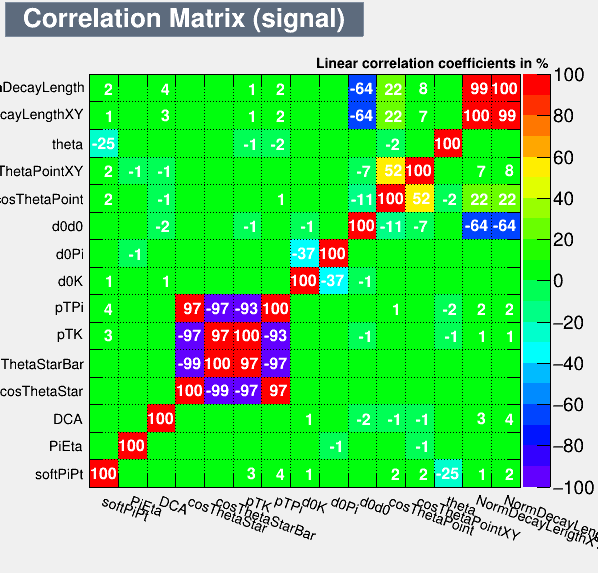
\includegraphics[width=0.48\textwidth]{training&testing/CorrelationMatrixSin.png}
        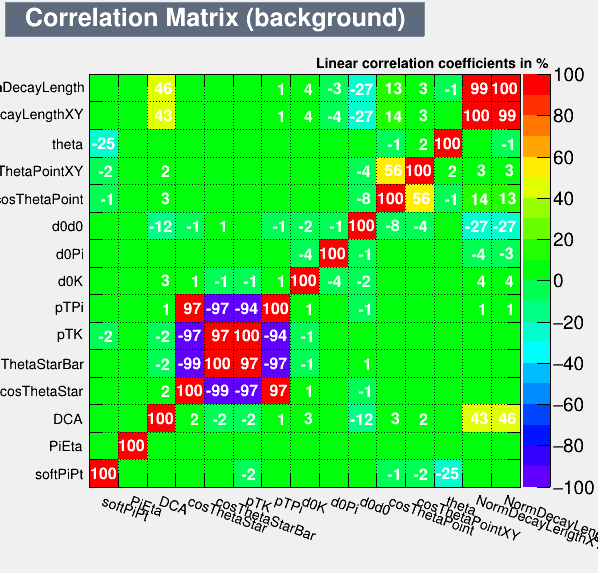
\includegraphics[width=0.48\textwidth]{training&testing/CorrelationMatrixBin.png}
       \caption{Correlazione lineare in percentuale tra le variabili discriminatorie del primo set per il training del segnale e del fondo.}
       \label{fig:correlazioneIn}
   \end{figure} 
    
 
    
    Dalle figure \ref{fig:CorrelazioneF} si vede che la correlazione supera il $50 \%$ per alcune delle variabili. Questo \`e comprensibile se si considera che alcune delle variabili sono strettamente correlate, per esempio la lunghezza di decadimento \`e correlata alla sua proiezione sul piano trasverso. E' stato quindi individuato un insieme di variabili scorrelate da utilizzare per la fase di training come si pu\`o vedere in figura \ref{fig:CorrelazioneF}. Tale insieme comprende variabili topologiche scorrelate tra loro e le variabili relative all'identificazione di particelle. Le uniche variabili che presentano un certo grado di correlazione sono la proiezione della lunghezza di decadimento delle candidate $D^0$ sul piano trasverso alla direzione del fascio (NormDecaYLenghtXY), il prodotto delle distanze minime tra le traiettorie del $k^-$ e del $\pi^+$ (d0d0) e la distanza minima di approccio (DCA) ma si è ritenuta accettabile questa correlazione. 
 
    \begin{figure}
       \centering
       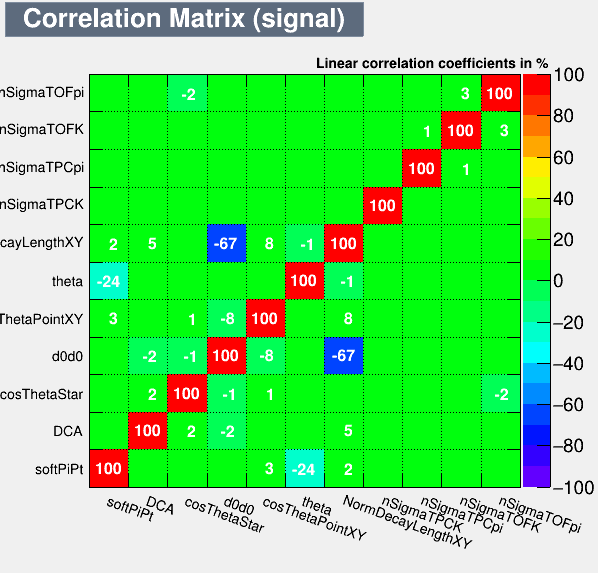
\includegraphics[width=0.48\textwidth]{training&testing/CorrelationMatrixS.png}
        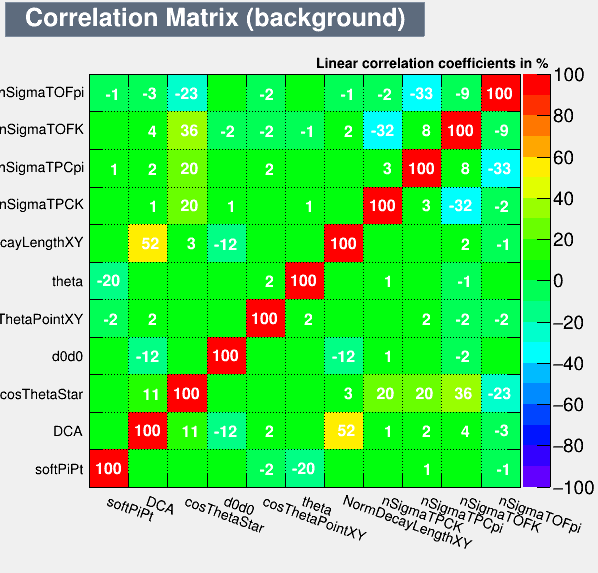
\includegraphics[width=0.48\textwidth]{training&testing/CorrelationMatrixB.png}
       \caption{Correlazione lineare in percentuale tra le variabili discriminatorie del secondo set per il training del segnale e per il training del fondo.}
       \label{fig:CorrelazioneF}
   \end{figure}
    
    

\subsection{Scelta dei parametri di configurazione del BDT}
Il TMVA permette di ottimizzare le performance dell'algoritmo scelto variando alcuni parametri di configurazione.

Il parametro utilizzato per valutare le performance dell'algoritmo \`e l'area sottesa alla curva chiamata \textit{Roc-Curve} (Receiving Operating Characteristics Curve). La Roc-Curve è il grafico della \textit{reiezione del fondo} in funzione dell'\textit{efficienza del segnale}. La reiezione del fondo è data da (1  -  efficienza del fondo), dove l'efficienza del fondo è la frazione di eventi di fondo effettivamente selezionati come fondo. L'efficienza del segnale è la frazione di eventi segnale effettivamente selezionati come segnale. Un algoritmo è tanto più efficiente quanto più è alto il valore dell'area sottesa alla Roc-Curve.  In figura \ref{fig:RocCurve} è riportata la curva della Roc-Curve per l'intervallo di $p_T$ [3-4] GeV/c. 

\begin{figure}[htbp] 
        \centering
        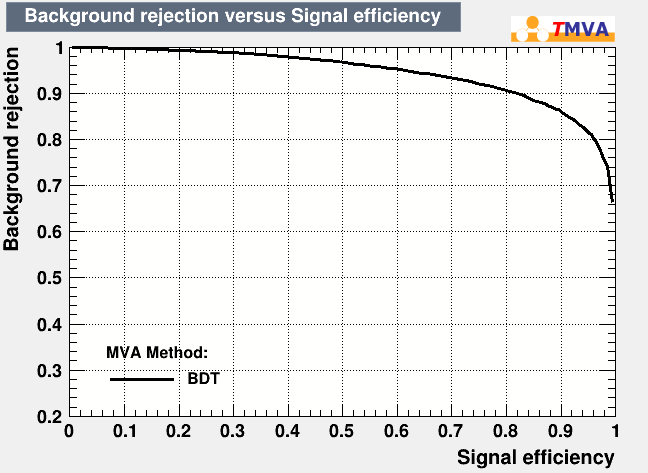
\includegraphics[width=0.7\linewidth]{training&testing/RocCurve.png}
        \caption{Grafico della Roc-Curve relativa al training del BDT per l'intervallo di $p_T$ [3,4] $GeV/c$}
        \label{fig:RocCurve}
    \end{figure}
    
Per determinare la migliore configurazione del BDT (in termini di accuratezza del training e tempo di esecuzione dell'algoritmo) da utilizzare per l'analisi in questa tesi sono stati variati due parametri:
    \begin{itemize}
        \item \textit{numero di alberi decisionali} che compongono la "foresta". Come spiegato nel paragrafo \ref{BDT} il training viene effettuato su un grande numero di alberi decisionali il cui responso viene unito in un'unica variabile discriminatoria finale. In generale, all'aumentare del numero di alberi decisionali l'efficienza dell'algoritmo migliora, ma aumenta anche il tempo necessario sia per il training che per l'applicazione del BDT. Questo accade a causa del maggior numero di alberi decisionali da considerare sia nella fase di training sia nella fase di applicazione dell'algoritmo. Si sono fatti alcuni tentativi per cercare un buon compromesso tra le performance dell'algoritmo e il tempo impiegato per analizzare i dati.  Nella tabella \ref{Tab:trees} si riporta il valore dell'area sottesa alla ROC-Curve al variare del numero di alberi decisionali considerati per il training, considerando come esempio l'intervallo di $p_T$ [3-4] GeV/c.
       
        \begin{table}[H]
		\centering
		\captionof{table}{Roc-Curve in funzione del numero di alberi decisionali nell'intervallo di $p_T$ [3-4] GeV/c\label{Tab:trees}}
		\begin{tabular}{c|c}
		    \toprule
		    N. di alberi decisionali &  area ROC-Curve  \\
            \midrule
              50 &   0.940 \\ 
           	 300 &   0.945 \\
             850 &   0.947 \\ 
			\bottomrule
		\end{tabular}
	\end{table}
	
	Per l'analisi svolta in questa tesi è stato utilizzato un BDT con 300 alberi, in quanto si è ritenuto di avere il maggior guadagno considerando sia il tempo necessario per il training e per l'applicazione del BDT che le performance dell'algoritmo.
	
	\item \textit{profondità massima} di ciascun albero decisionale del BDT. La profondità di un albero decisionale è il numero di livelli di cui è composto l'albero stesso, ovvero il numero di diramazioni. Come per il numero di alberi decisionali, in generale se si aumenta la profondità massima migliorano le performance dell'algoritmo, ma aumenta il tempo necessario per la fase di training e di applicazione dell'algoritmo di BDT.
	Nella tabella \ref{Tab:profondità} è riportata l'area sottesa alla ROC-Curve per i valori di profondità considerati, per il training fatto con 300 alberi considerando come esempio l'intervallo di $p_T$ [3,4] GeV/c.
	
	\begin{table}[H]
		\centering
		\captionof{table}{Roc-Curve in funzione della profondit\`a massima per l'intervallo di $p_T$ [3,4] GeV/c.\label{Tab:profondità}}
		\begin{tabular}{c|c}
		    \toprule
		    profondità  &  area Roc-Curve  \\
            \midrule
           	 2 &   0.924  \\ 
             3 &   0.945 \\
             4 &   0.947 \\ 
			\bottomrule
		\end{tabular}
	\end{table}
    Si è ritenuto che l'opzione migliore, considerando sia il tempo necessario per l'analisi dati sia le performance dell'algoritmo, fosse di considerare alberi con profondità massima di 3 nell'analisi svolta in questa tesi.
    \end{itemize}

\section{I risultati del Training}
Una volta identificato il campione da usare come segnale e fondo, le variabili discriminatorie scorrelate da fornire come input al modello e la configurazione del BDT si è proceduto con la fase di training. 
\\L'algoritmo di analisi multivariata analizza le variabili discriminatorie per fornire un unico valore di output che permette di separare il segnale dal fondo, che nel resto del capitolo sarà chiamato \textit{BDT response}. Il grafico in figura \ref{fig:BDTresponse} mostra la distribuzione del BDT response calcolato per il campione di segnale (blu) e per il fondo (rosso) normalizzate allo stesso numero di eventi. Nella figura si vede che le distribuzioni del segnale e del fondo sono ben distinte e che solo nell'intervallo $-0.3 < BDT response < 0.25$ il fondo si sovrappone parzialmente al segnale. 
    \begin{figure}[htbp] 
        \centering
        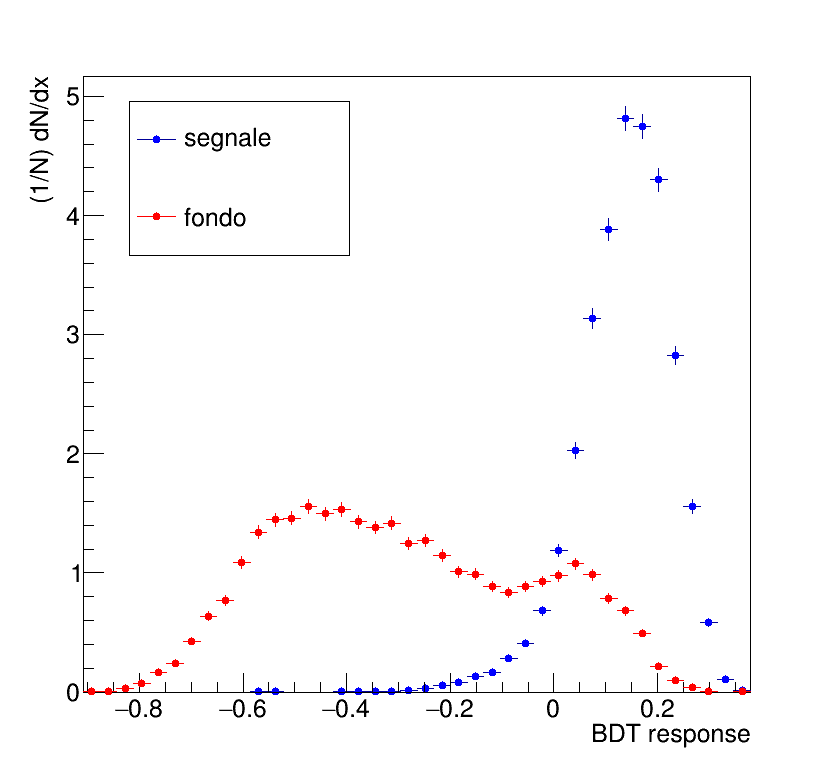
\includegraphics[width=0.7\linewidth]{training&testing/distribuzioneBDT_test.png}
        \caption{Distribuzione della variabile discriminatoria (BDT response). In blu la distribuzione relativa al segnale e in rosso quella relativa al fondo combinatoriale per l'intervallo di $p_T$ [3,4] GeV/c. Le distribuzioni sono state normalizzate allo stesso numero di eventi.} 
        \label{fig:BDTresponse}
    \end{figure}
    
    
Sia l'efficienza di selezione del segnale sia quelle di selezione del fondo variano al variare del BTD response come mostrato in figura \ref{fig:efficienza}. Inoltre, nella stessa figura e' mostrata la curva della significanza definita come:
    \begin{equation}
        sign \ = \ \frac{segnale}{\sqrt{segnale + fondo}}
    \end{equation}

    \begin{figure}[htbp] 
        \centering
        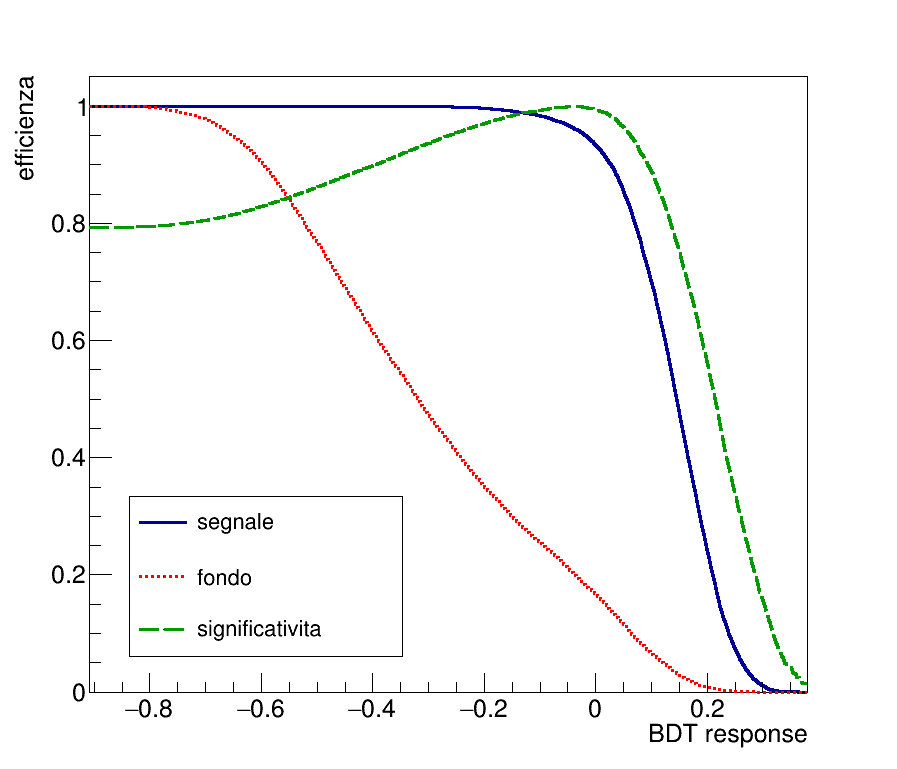
\includegraphics[width=0.7\linewidth]{training&testing/eff_significanza.png}
        \caption{Efficienza di selezione del segnale in blu, del fondo in rosso e significanza in verde in funzione del valore della variabile BDT response per il training effettuato nell'intervallo di $p_T$ [3,4] GeV/c }
        \label{fig:efficienza}
    \end{figure}

\section{Testing} \label{testing}
    Una parte del campione di cui è nota la divisione tra segnale e fondo viene utilizzata per la fase di verifica del training stesso, detta \textit{fase di test}. 
    \\In questa fase si vuole controllare che non ci sia stato \textit{overtraining} durante la fase di training, ovvero che il BDT si sia adattato eccessivamente al campione di dati del training e non sia più descrittivo del fenomeno fisico che si vuole considerare nella  sua generalità. Se non c'è stato overtraining, ci si aspetta che la distribuzione del BDT response sia la stessa per i dati del training e quelli del test. 
    \\In tabella \ref{Tab:test} è riportata la quantità di dati utilizzata per il test per ogni intervallo di $p_T$ considerato.
    
    \begin{table}[H]
		\centering
		\captionof{table}{Campione di dati utilizzato per il la fase di test\label{Tab:test}}
		\begin{tabular}{c|c|c}
		    \toprule
		    intervallo $p_T$ [GeV/c]  &  quantità di dati testing segnale & quantità di dati testing fondo  \\
            \midrule
            1 - 2  	&  3165   &  37853  \\ 
            2 - 3 	&  11560   &  26498  \\
            3 - 4  	&  14395   &  14743  \\ 
            4 - 5  	&  13292   &  6090 \\ 
            5 - 6  	&  5868   &  1076  \\ 
            6 - 8  	&  6301   &  719  \\ 
            8 - 12  &  5589   &   464 \\   
			\bottomrule
		\end{tabular}
	\end{table}
    
    In figura \ref{fig:testing_3_4} è riportata la distribuzione della variabile BDT response per il campione di dati utilizzati nella fase di training e in quella di test per l'intervallo di $p_T$ [3,4] GeV/c. Dalla figura si vede che le due distribuzioni sono compatibili entro gli errori statistici e pertanto si verifica che non c'è stato overtraining.
    
    
    \begin{figure}[htbp] 
        \centering
        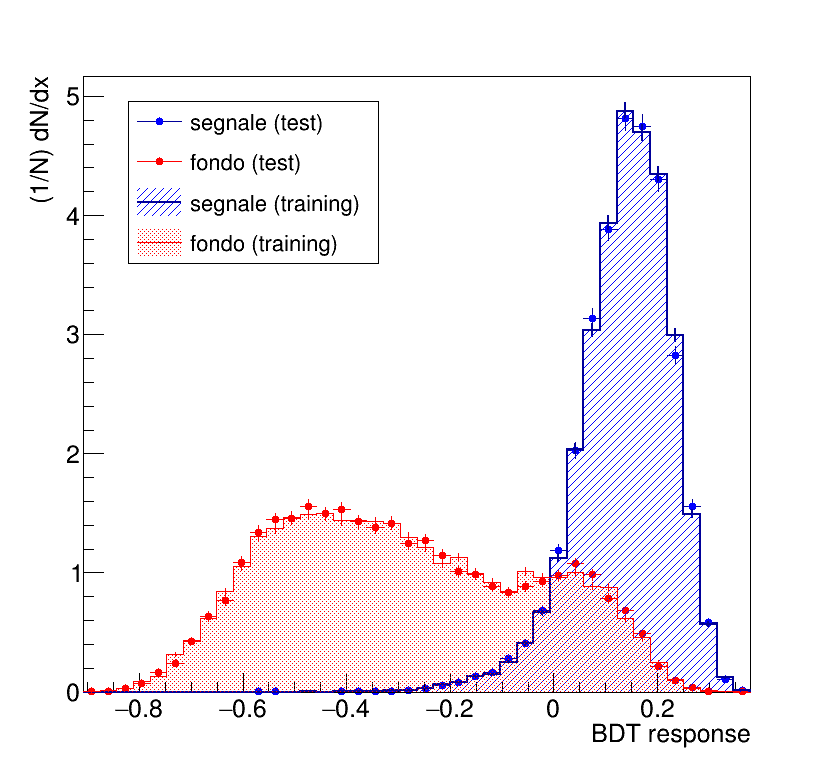
\includegraphics[width=0.7\linewidth]{training&testing/distribuzione_test_train.png}
        \caption{Distribuzione del BDT response per il campione di dati utilizzato per la fase di training (area tratteggiata) e per la fase di test (punti) per l'intervallo di $p_T$ [3,4] GeV/c, in rosso per il fondo e in blu per il segnale}
        \label{fig:testing_3_4}
    \end{figure}
 
    %In figura \ref{fig:testing_6_8} si vede la distribuzione del BDT response per il campione di dati del training e del testing per l'intervallo di $p_T$ [6,8] GeV/c. Si vede che le distribuzioni per il training e per il testing sono compatibili per la maggior parte dei valori del BDT response ma non in tutti come nel caso dell'intervallo di $p_T$ [3,4]. In generale i grafici della distribuzione del BDT response per il campione dati del training e del testing per i vari intervalli di $p_T$ considerati mostrano che al crescere del $p_T$ le distribuzioni per il campione del test e del training sono sempre meno compatibili, 
 
    %\begin{figure}[htbp] 
     %   \centering
      %  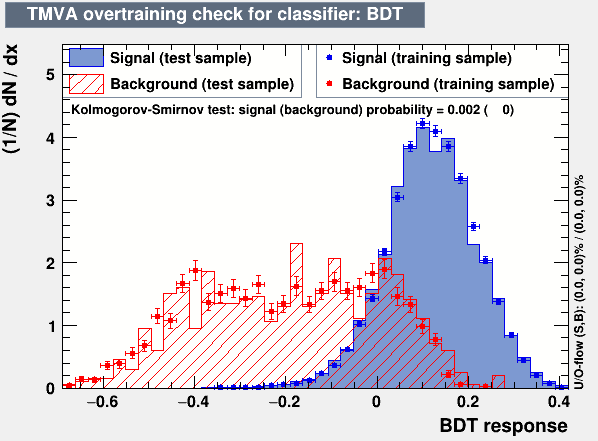
\includegraphics[width=0.7\linewidth]{training&testing/overtraining_6_8.png}
     %   \caption{Distribuzione del BDT response per il training (punti e relativi errori) e per il testing (rettangoli) per il bin di $p_T$ [6,8] GeV/c, in rosso i dati del fondo e in blu quelli relativi al segnale}
     %   \label{fig:testing_6_8}
    %\end{figure}
 
    %I grafici \ref{fig:testing_3_4} e \ref{fig:testing_6_8} mostrano che non c'è stato overtraining, pertanto si può procedere con l'analisi dei dati.




\section{Scelta dei valori di taglio}

Ottenute le distribuzioni del BDT response e gli andamenti delle efficienze e della significanza per i vari intervalli di $p_T$ considerati, si sono individuati i valori di taglio del BDT response per  discriminare tra segnale e fondo nella fase di applicazione del BDT. 
\\Per scegliere il valore di taglio della variabile di output del BDT per separare segnale e fondo si sono provate due diverse opzioni:
    \begin{itemize}
    \item $taglio \ a$: il punto di massimo della significanza, calcolata con un'opportuna scelta del rapporto segnale su fondo;
    \item $taglio \ b$: punto in cui la distribuzione del BDT response per il segnale e per il fondo si incrociano %un valore più basso di $0.1$ del punto di massimo della significatività.
    \end{itemize}
La tabella \ref{Tab:tagli} riporta i valori del taglio presi in considerazione per ogni intervallo di $p_T$.

\begin{table}[H]
		\centering
		\captionof{table}{Valori del taglio del BDT response\label{Tab:tagli}}
		\begin{tabular}{c|c|c}
		    \toprule
		    intervallo di $p_T$ [GeV/c]  &  valore del $taglio \ a$ & valore del $taglio \ b$ \\
            \midrule
           	1 - 2  	&    0.049  &   0.148\\ 
            2 - 3 	&    0.045  &   0.146\\ 
            3 - 4  	&    0.031  &   0.133\\ 
            4 - 5  	&    0.027  &   0.127\\ 
            5 - 6  	&    0.031  &   0.130\\ 
            6 - 8  	&    0.034  &   0.132\\ 
            8 - 12  &    0.105  &   0.201\\   
			\bottomrule
		\end{tabular}
	\end{table}
	
In un primo momento l'applicazione del BDT ai dati è stata effettuata con entrambe le possibilità di valori di taglio per il BDT response e si è visto che entrambe permettevano di selezionare le candidate $D^{*+}$ e di ottenere il picco di segnale. Si \`e scelto di continuare l'analisi considerando solamente il valore di taglio più basso (taglio b) in quanto permette di preservare una quantit\`a maggiore di segnale.  

%Nell'utilizzare i grafici di efficienze e significatività per la scelta del valore di taglio è stato fondamentale aver considerato un rapporto segnale-fondo molto basso (10:1000), questo perchè nei dati di ALICE abbiamo che gli eventi segnale sono molti meno degli eventi fondo. In tal modo anche i risultati del training del BDT e le curve di efficienze e significatività sono più aderenti ai dati di ALICE.

  %  \begin{figure}[htbp] 
   %     \centering
  %      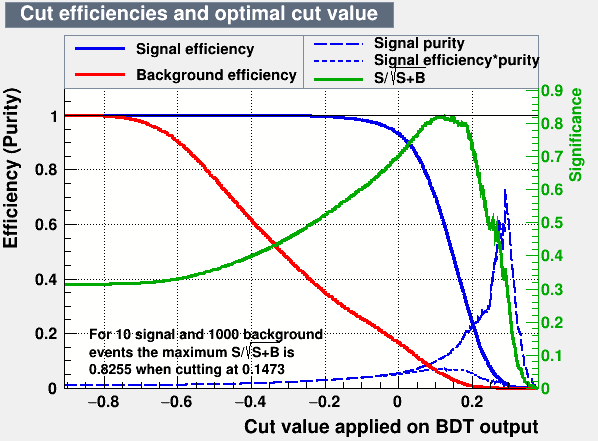
\includegraphics[width=0.7\linewidth]{training&testing/effBDT/effBDT_rapp_3_4.png}
  %      \caption{Grafico dell'efficienza del segnale in blu, efficienza del fondo in rosso e significatività in verde, al variare del valore del taglio scelto per la BDTresponse per il bin di $p_T$ [3,4]. Il rapporto tra segnale e fondo è di 10:1000 . Gli andamenti sono relativi al training con 300 alberi e profondità massima 3
   %     }
   %     \label{fig:effBDT_10_1000}
   % \end{figure}
  
  
